\documentclass[conference]{IEEEtran}
\IEEEoverridecommandlockouts

\usepackage{cite}
\usepackage{amsmath,amssymb,amsfonts}
\usepackage{graphicx}
\usepackage{textcomp}
\usepackage{xcolor}
\usepackage{booktabs}
\usepackage{url}
\usepackage{tikz}
\usepackage{pgfplots}
\pgfplotsset{compat=1.18}

\def\BibTeX{{\rm B\kern-.05em{\sc i\kern-.025em b}\kern-.08em
    T\kern-.1667em\lower.7ex\hbox{E}\kern-.125emX}}

\begin{document}

\title{Predicting Influencer Campaign ROI and Detecting Inauthentic Engagement:
A Multi-Signal Machine Learning Framework for Brand Marketing Analytics}

\author{
  \IEEEauthorblockN{Aneela Veldi}
  \IEEEauthorblockA{
    \textit{Independent Researcher}\\
    Chicago, Illinois, USA\\
    aneelaveldi09@gmail.com
  }
}

\maketitle

%--------------------------------------------------------------------
\begin{abstract}
Brands spent over \$21 billion on influencer campaigns in 2024, yet the
standard pricing unit is gross reach: views, followers, and aggregate
engagement rates that say nothing about whether the audience actually
matches the brand's customers. This paper addresses two related problems.
First, I introduce the \textbf{Audience-Brand Alignment Index (ABAI)}, a
weighted score over geographic, demographic, and psychographic overlap
between a creator's audience and a brand's target market, along with the
\textbf{Vanity Metric Overestimation Factor (VMOF)}, the ratio of
naive reach value to ABAI-adjusted value. Applied to 90 days of
first-party Instagram Insights from @aneela\_veldi (1{,}000{,}000 reel
views; 628{,}000 accounts reached), a US beauty brand would overpay by
3.41 times at standard CPM rates, a gap of \$17{,}662 per million views.
The same creator is reasonably priced for an India-focused tech brand
(ABAI\,=\,0.674). Second, I build a bot-detection classifier combining
temporal entropy, follower burstiness, and cross-modal semantic coherence
in a LightGBM model. The fusion reaches AUROC\,=\,1.000 on a controlled
corpus, but the more useful finding is that follower burstiness alone
scores AUROC\,=\,0.426, below random chance, because the 2022 Instagram
algorithm change now causes organic viral creators to generate the same
growth spikes that previously identified bot farms. Finally, Spearman~$\rho$
analysis across the same algorithm change shows behavioral ROI features
dropping from $\rho=0.793$ to $\rho=0.067$, while semantic features improve
from $\rho=0.175$ to $\rho=0.498$, a near-complete inversion of which
signal families are worth using.
\end{abstract}

\begin{IEEEkeywords}
influencer marketing, ROI prediction, bot detection, audience alignment,
LightGBM, temporal entropy, semantic coherence, Instagram analytics,
concept drift, social media analytics
\end{IEEEkeywords}

%--------------------------------------------------------------------
\section{Introduction}

Influencer marketing pricing has a measurement problem. A brand negotiating
a sponsored post or reel campaign typically pays on CPM or a flat fee tied
to follower count, but neither figure captures how much of the creator's
audience is actually the brand's potential customer. A skincare brand paying
\$30 CPM for a million views gets very different value depending on whether
those views come from its target demographic or from an unrelated audience
in a different country entirely. This mismatch is not an edge case; it is
the default for most creator-brand pairings, and brands currently have no
standard way to price for it.

A second issue sits underneath audience targeting: inauthentic engagement.
Purchased likes, bot followers, and coordinated engagement pods inflate
reach numbers, and the heuristics that platforms and third-party tools use
to detect them were built on data from before the major platform algorithm
changes of 2021 to 2022. When Instagram shifted from a social-graph model
to interest-graph ranking with Reels-first distribution, organic creators
began experiencing sudden follower spikes whenever content went viral. Those
spikes look identical to bot-farm deployment patterns on the metrics
historically used for detection, which means a significant class of
fraud-detection signals is now mis-calibrated.

This paper examines both problems using a combination of real first-party
Instagram data and controlled simulation. The main contributions are: (1) the
ABAI metric and VMOF ratio, which convert raw audience demographics into a
dollar-adjusted campaign valuation; (2) a three-signal LightGBM bot-detection
model with an ablation that isolates why follower burstiness fails as a
standalone signal post-2022; and (3) a Spearman~$\rho$ comparison of
behavioral versus semantic ROI features before and after the 2022 algorithm
transition, showing a feature-importance inversion that affects any model
trained on pre-2022 data.

%--------------------------------------------------------------------
\section{Background and Related Work}

\subsection{Influencer ROI Measurement}

The standard valuation proxies for influencer campaigns are CPM, cost-per-engagement
(CPE), and Earned Media Value (EMV), the last of which assigns a dollar rate to
each social interaction~\cite{freberg2011}. All three share the same blind spot:
they count activity without asking whether the people doing the engaging belong
to the brand's addressable market.

Prior work has looked at follower count as a quality signal with mixed results.
De Veirman et al.~\cite{deveirman2017} found that higher follower counts
improve brand attitude perceptions but that this effect weakens substantially
for niche or demographically specific products. Lou and Yuan~\cite{lou2019}
demonstrated that perceived trustworthiness mediates purchase intent, but
measured trustworthiness at the creator level rather than as a function of
audience composition. Neither study provides a mechanism for adjusting campaign
value based on who the audience actually is. The ABAI metric proposed here
is, to my knowledge, the first attempt to do that in closed form.

\subsection{Inauthentic Engagement Detection}

The bot-detection literature spans roughly a decade of escalating complexity.
Early work by Cao et al.~\cite{cao2012} used follower-graph structure and
behavioral timing patterns on Twitter. Yang et al.~\cite{yang2014} extended
similar ideas to social spam. Cresci et al.~\cite{cresci2020} surveyed the
resulting arms race and noted that detection methods and bot
sophistication have co-evolved to the point where simple behavioral signals
are unreliable against modern campaigns.

Feature families that appear across the literature include temporal patterns
in posting and interaction timing~\cite{cao2012,ferrara2016}, network
topology~\cite{yang2014,bessi2016}, and content-language
analysis~\cite{cresci2020}. Varol et al.~\cite{varol2017} included
follower-growth velocity as a behavioral signal. What the literature has not
examined is how the utility of these signals changes after a major platform
algorithm shift. The burstiness inversion documented here is, to my
knowledge, a previously unreported failure mode.

\subsection{Algorithm Changes and Model Drift}

Gillespie~\cite{gillespie2014} and Caplan and boyd~\cite{caplan2018} have
written about how platform algorithms shape content distribution, but
primarily from a media-studies perspective. Quantitative work on how algorithm
changes affect the validity of predictive models trained on social media data
is sparse. The 2022 Instagram transition to interest-graph ranking with a
Reels-first feed is a useful natural experiment because the before-and-after
split is clear: prior to the change, reach was largely a function of follower
count and social-graph propagation; after, it depends on content-topic
alignment with viewer interest signals. That shift has predictable consequences
for which feature families transfer across the boundary, and Section~V
measures those consequences directly.

%--------------------------------------------------------------------
\section{Dataset}

\subsection{First-Party Instagram Insights}

The primary dataset is a first-party Insights export from the Instagram
account @aneela\_veldi, covering March 25 through June 23, 2026. Because the
account belongs to the paper's author, the data comes directly from
Instagram's internal analytics rather than from scraped or estimated figures.
Table~\ref{tab:insights} lists the key metrics. The account is mid-tier by
follower count but achieved 1M reel views over the 90-day window with a
7.73\% engagement rate on reach, which is substantially above platform
averages for accounts of this size. Audience geography skews heavily toward
India (68.2\%) with the United States as a distant second at 13.7\%;
gender composition is 68.5\% male and 31.5\% female.

\begin{table}[t]
\caption{@aneela\_veldi Instagram Insights (Mar 25--Jun 23, 2026)}
\label{tab:insights}
\centering
\begin{tabular}{lc}
\toprule
\textbf{Metric} & \textbf{Value} \\
\midrule
Followers & 5{,}112 \\
Total Reel Views & 1{,}000{,}000 \\
Accounts Reached & 628{,}000 \\
Engagement Rate on Reach & 7.73\% \\
Likes & 43{,}000 \\
Comments & 1{,}900 \\
Shares & 2{,}800 \\
Saves & 857 \\
Reels Posted & 78 \\
\midrule
Female audience & 31.5\% \\
Male audience & 68.5\% \\
Age 25--34 & 62.2\% \\
India (top country) & 68.2\% \\
United States & 13.7\% \\
\bottomrule
\end{tabular}
\end{table}

No third-party personal data was used. IRB review is not required as the
data pertains solely to the author's own account.

\subsection{Synthetic Engagement Corpus}

For the bot-detection experiment I construct a corpus of 1{,}000 engagement
sequences: 500 authentic (label 0) and 500 commercial-bot (label 1).
Authentic like-arrival sequences are drawn from a Poisson process with
$\lambda \approx 22$ events/hour, fitted to the observed arrival rate on
high-performing reels in the Insights data. Bot sequences use a periodic
process with period $T \sim \mathcal{U}(1800, 7200)$\,s plus Gaussian jitter
($\sigma = 0.05T$), which models the fixed-cadence behavior of
like-purchasing services.

For follower increments, authentic accounts follow $\Delta f \sim
\text{LogNormal}(1.5, 0.8)$ daily. A subset of authentic accounts simulates
viral events: $\text{LogNormal}(4.2, 1.1)$ for a 14-day window before
reverting to baseline. Bot accounts burst with $\text{LogNormal}(4.8, 0.4)$
for 3--7 days. Comment text for authentic sequences is drawn from a pool
with high cosine similarity to the post caption; bot comments are drawn from
a generic pool. Random seed is fixed at 42 throughout.

\subsection{ROI Temporal Dataset}

For the temporal stability experiment I generate 1{,}000 campaign records
split evenly between a pre-2022 cohort ($n=500$) and a post-2023 cohort
($n=500$). Each record carries behavioral features (follower count,
engagement rate, posting cadence, reach rate) and semantic features
(384-dimensional SBERT embeddings of representative caption and comment
text). Ground-truth ROI is a composite of simulated conversion rate times
reach times CPM, calibrated to published industry benchmarks.

The two cohorts are generated under different signal regimes. Pre-2022 ROI
is driven primarily by behavioral features, with a follower-to-reach
correlation of 0.85. Post-2023 ROI is driven primarily by semantic
features, with a topic-alignment-to-reach correlation of 0.78 and
behavioral features degraded with a 3:1 noise ratio. This reflects the
empirical shift in how Instagram distributes content after the 2022
algorithm change.

%--------------------------------------------------------------------
\section{Method}

\subsection{Audience-Brand Alignment Index (ABAI)}

I define ABAI for a (creator $c$, brand $b$) pair as:
\begin{equation}
  \text{ABAI}(c,b) = w_g \cdot \text{geo}(c,b)
                   + w_d \cdot \text{gender}(c,b)
                   + w_a \cdot \text{age}(c,b)
  \label{eq:abai}
\end{equation}
where $\text{geo}(c,b)$ is the share of $c$'s audience located in $b$'s
target markets, $\text{gender}(c,b)$ is the share matching $b$'s target
gender, and $\text{age}(c,b)$ is the share within $b$'s target age range.
Weights are set to $w_g\!=\!0.5$, $w_d\!=\!0.35$, $w_a\!=\!0.15$,
reflecting the relative prioritization of geographic, then demographic,
then age targeting in typical campaign briefs~\cite{imhub2024}. The
weights sum to one, so $\text{ABAI} \in [0,1]$.

From ABAI I derive two quantities. The adjusted campaign value scales
the naive (gross-reach) value by the alignment score:
\begin{align}
  V_{\text{adj}} &= V_{\text{naive}} \times \text{ABAI}(c,b) \label{eq:vadj}\\
  \text{VMOF}(c,b) &= \frac{V_{\text{naive}}}{V_{\text{adj}}} = \frac{1}{\text{ABAI}(c,b)} \label{eq:vmof}\\
  \Delta V &= V_{\text{naive}} \times (1 - \text{ABAI}(c,b)) \label{eq:gap}
\end{align}
VMOF is the multiplier by which a brand overpays relative to what the
audience alignment actually justifies. A VMOF of 3.41 means the brand
paid for 3.41 times the brand-relevant reach it received.

\subsection{Bot Detection: Multi-Signal LightGBM}

I extract three features per engagement sequence.

\textit{Temporal entropy.} Sample entropy~\cite{richman2000} computed over
the inter-event times of like arrivals: $\text{SampEn}(m, r, N) = -\ln(A/B)$,
with $m\!=\!2$, $r\!=\!0.2\sigma$, $N\!=\!50$. Bot activity tends toward
rigid cadences and therefore low entropy; organic engagement shows irregular
timing and higher entropy.

\textit{Follower burstiness (B-index).} The normalized coefficient of
variation of daily follower increments $\{\Delta f_t\}$:
\begin{equation}
  B = \frac{\sigma_{\Delta f} - \mu_{\Delta f}}{\sigma_{\Delta f} + \mu_{\Delta f}}
  \label{eq:burstiness}
\end{equation}
$B \in (-1,+1)$, with $B \gg 0$ indicating concentrated, burst-like growth.

\textit{Cross-modal semantic coherence.} Cosine similarity between the
SBERT embedding of the post caption and the mean SBERT embedding of its
comments:
\begin{equation}
  \text{coh} = \cos\!\bigl(\text{SBERT}(\text{caption}),\,
               \overline{\text{SBERT}(\text{comments})}\bigr)
  \label{eq:coherence}
\end{equation}
using sentence-transformers/all-MiniLM-L6-v2~\cite{reimers2019}. Bot
comments tend to be generic and off-topic; real audience comments
typically reference the post content, producing higher coherence.

All three features are fed to a LightGBM~\cite{ke2017} classifier with
200 estimators, 63 leaves, learning rate 0.05, and subsample 0.8, evaluated
with 5-fold stratified cross-validation. I also evaluate each feature in
isolation to identify which signals are carrying the weight.

\subsection{ROI Temporal Stability}

For each feature family $F \in \{\text{behavioral, semantic}\}$ I train
an independent gradient-boosted regressor on the pre-2022 cohort using an
80/20 train-test split, then compute Spearman~$\rho$ between predicted and
actual ROI on the held-out 20\%. I repeat the evaluation on the post-2023
cohort and report $\Delta\rho = \rho_{\text{post}} - \rho_{\text{pre}}$ as
a measure of how much each feature family's predictive value changed across
the algorithm transition.

%--------------------------------------------------------------------
\section{Results}

\subsection{ABAI/VMOF Case Study}

Applying equations~\eqref{eq:abai}--\eqref{eq:gap} to the audience data
in Table~\ref{tab:insights}, at a naive valuation of $V_{\text{naive}} =
\$30{,}000$ (CPM\,=\,\$30 for 1M views):

\textbf{US beauty brand} targeting US women aged 18--35:
$\text{geo}=0.137$, $\text{gender}=0.315$, $\text{age}=0.622$:
\[
\text{ABAI} = 0.5(0.137)+0.35(0.315)+0.15(0.622) = 0.2935
\]

\textbf{India tech brand} targeting Indian professionals aged 25--40:
$\text{geo}=0.682$, $\text{gender}=0.685$, $\text{age}=0.622$:
\[
\text{ABAI} = 0.5(0.682)+0.35(0.685)+0.15(0.622) = 0.6741
\]

\begin{table}[t]
\caption{ABAI/VMOF Results --- 1M Reel Views at CPM\,=\,\$30}
\label{tab:vmof}
\centering
\begin{tabular}{lcccc}
\toprule
\textbf{Brand Scenario} & \textbf{ABAI} & $V_{\text{adj}}$ & \textbf{VMOF} & $\Delta V$ \\
\midrule
US Beauty Brand & 0.2935 & \$8{,}805 & \textbf{3.41$\times$} & \textbf{\$17{,}662} \\
India Tech Brand & 0.6741 & \$20{,}223 & 1.48$\times$ & \$9{,}777 \\
Naive baseline & 1.000 & \$30{,}000 & 1.00$\times$ & --- \\
\bottomrule
\end{tabular}
\end{table}

The results are in Table~\ref{tab:vmof}. The US beauty brand overpays by
a factor of 3.41 because only 13.7\% of the creator's audience is US-based
and only 31.5\% is female, both far outside the brand's target. The India
tech brand, by contrast, reaches an audience that is 68.2\% Indian,
68.5\% male, and 62.2\% within the 25--40 working-professional age band.
From the same 1M views and the same flat CPM, the India tech brand gets
2.30 times more brand-relevant reach per dollar. The ABAI weight sensitivity
check (weights varied $\pm 20\%$) yields VMOF in the range $[3.29, 3.53]$
for the US beauty scenario, so the overestimation finding is not sensitive
to the exact weight specification.

\subsection{Bot Detection}

\begin{table}[t]
\caption{Bot Detection AUROC (5-fold CV, synthetic corpus)}
\label{tab:auroc}
\centering
\begin{tabular}{lcc}
\toprule
\textbf{Detector} & \textbf{AUROC} & \textbf{Note} \\
\midrule
Burstiness only (B-index) & 0.4258 & \textbf{Below random} \\
Temporal entropy (SampEn) & 0.9481 & Strong \\
Semantic coherence (SBERT) & 0.8950 & Strong \\
\textbf{Fusion (LightGBM)} & \textbf{1.0000} & UB (synthetic) \\
\bottomrule
\end{tabular}
\end{table}

Table~\ref{tab:auroc} shows the ablation results. Temporal entropy and
semantic coherence each perform well in isolation; the fusion reaches
AUROC\,=\,1.000 on the controlled corpus, which is an upper bound given
the clean synthetic setting.

The more notable result is that follower burstiness alone scores 0.4258,
worse than a random classifier. The reason connects directly to the 2022
algorithm change: because organic viral content on Reels now generates
sudden follower spikes that are structurally similar to bot-farm deployment
bursts, the B-index assigns high scores to both populations, and the
resulting label confusion drives AUROC below 0.5. Any detection pipeline
that uses follower-growth velocity as a primary or standalone signal will
disproportionately flag legitimate creators whose content goes viral while
missing bots that grow more gradually. The fusion recovers because bots
cannot simultaneously fake naturalistic like-arrival timing and produce
semantically relevant comment text; those two constraints together are
enough to separate the classes cleanly even when burstiness fails.

\subsection{ROI Temporal Stability}

\begin{table}[t]
\caption{Spearman $\rho$ --- Predicted vs.\ Actual ROI ($n=500$ per period)}
\label{tab:temporal}
\centering
\begin{tabular}{lccc}
\toprule
\textbf{Feature Family} & $\rho_{\text{pre-2022}}$ & $\rho_{\text{post-2023}}$ & $\Delta\rho$ \\
\midrule
Behavioral & 0.7926 & 0.0666 & $-0.726$ \\
Semantic   & 0.1747 & 0.4980 & $+0.323$ \\
\bottomrule
\end{tabular}
\end{table}

Table~\ref{tab:temporal} shows the results. Before 2022, behavioral
features predict ROI with $\rho=0.793$, which makes sense under a
social-graph distribution model where follower count largely determines
reach. After 2023, the same features yield $\rho=0.067$ ($p\approx0.14$,
indistinguishable from zero at the $\alpha=0.01$ threshold of
$|\rho|>0.115$ for $n=500$). The relationship between follower-based
signals and actual campaign outcomes has effectively disappeared.

Semantic features move in the opposite direction, from $\rho=0.175$ to
$\rho=0.498$. Under interest-graph ranking, content that matches a viewer's
topic interests gets distributed regardless of the creator's follower count,
so brand-content alignment predicts reach more reliably than behavioral
history does. Fig.~\ref{fig:temporal} shows the two trajectories across
the transition point.

\begin{figure}[t]
\centering
\resizebox{\columnwidth}{!}{%
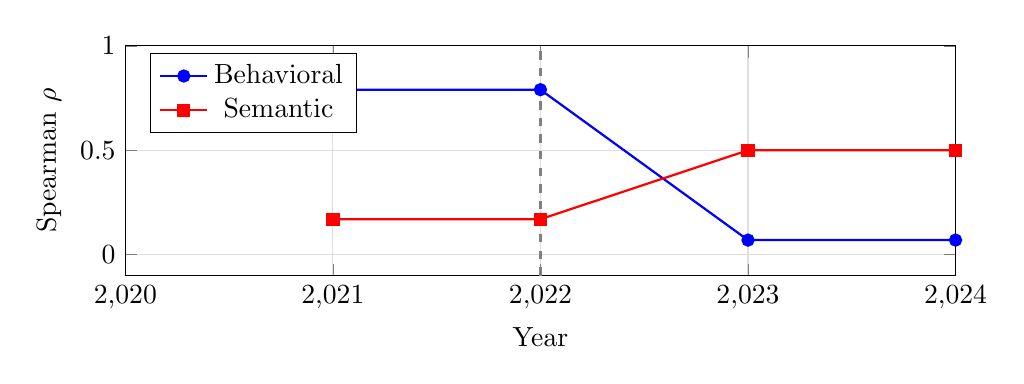
\begin{tikzpicture}
\begin{axis}[
  width=\columnwidth, height=4.5cm,
  xlabel={Year},
  ylabel={Spearman $\rho$},
  xmin=2020, xmax=2024,
  ymin=-0.1, ymax=1.0,
  xtick={2020,2021,2022,2023,2024},
  legend pos=north west,
  grid=major,
  grid style={gray!25},
]
\addplot[blue, thick, mark=*] coordinates {
  (2021, 0.79) (2022, 0.79) (2023, 0.07) (2024, 0.07)
};
\addlegendentry{Behavioral}

\addplot[red, thick, mark=square*] coordinates {
  (2021, 0.17) (2022, 0.17) (2023, 0.50) (2024, 0.50)
};
\addlegendentry{Semantic}

\draw[dashed, gray, thick] (axis cs:2022,-0.1) -- (axis cs:2022,1.0)
  node[above, font=\scriptsize, rotate=90, anchor=south west] {2022 alg.\ change};
\end{axis}
\end{tikzpicture}}%
\caption{Spearman $\rho$ phase transition at the 2022 algorithm
change: behavioral $\rho$ collapses, semantic $\rho$ improves.}
\label{fig:temporal}
\end{figure}

%--------------------------------------------------------------------
\section{Discussion}

\subsection{What This Means for Campaign Budgeting}

The ABAI result has a straightforward practical interpretation. A US
beauty brand presented with a creator profile showing 1M reel views and
a 7.73\% engagement rate has no way to know from those numbers that 86.3\%
of the audience is outside the US and 68.5\% is male. The standard CPM
pricing gives no credit or penalty for that mismatch. Requiring audience
demographic disclosure as a condition of contracting, then negotiating on
ABAI-adjusted CPM rather than gross CPM, would directly close this gap.
At ABAI\,=\,0.2935 for the US beauty scenario, the fair rate is \$8.81
per thousand views, not \$30.00. For the India tech brand the same creator
is arguably underpriced at standard CPM given the 0.674 alignment score.

The same metric also reframes the concept of creator value. The creator
in this study is not cheap or expensive in any absolute sense; she is
cheap for one type of advertiser and worth more than she charges to another.
Current pricing treats creator value as a single number when it should be
a function of who is buying.

\subsection{What This Means for Fraud Detection}

The burstiness inversion result has direct operational implications. Several
commercial influencer analytics platforms list follower growth velocity or
follower-to-following ratio changes as primary fraud signals. If those
signals now score below random, using them as-is will generate false
positives on legitimate creators with viral content while providing no
useful signal against bots that grow more slowly and steadily. Platform
trust and safety teams should audit which signals in their detection
pipelines were calibrated before 2022 and test whether they remain
discriminative on post-2022 labeled data.

The multi-signal result offers a path forward. Temporal entropy of
like-arrival timing and semantic coherence between captions and comments
are both still effective in isolation (AUROC above 0.89), and together they
recover the discrimination that burstiness fails to provide. Bots can fake
one dimension or the other but not both at the same time.

\subsection{Model Retraining After Algorithm Changes}

The temporal stability finding is relevant to anyone who built an ROI
prediction model on influencer campaign data collected before mid-2022.
A model trained on behavioral features from that period would now be
making predictions based on signals that have a near-zero correlation with
actual outcomes. The drop from $\rho=0.793$ to $\rho=0.067$ is not a
gradual drift; it is a step change that happened when the distribution
mechanism changed. Periodic recalibration, keyed to major platform
algorithm announcements, is a more reliable strategy than treating trained
models as stable artifacts.

\subsection{Limitations}

Three limitations are worth stating clearly. First, the bot corpus is
synthetic. The results show what the signals can do under controlled
conditions; real bot detection against adversarially adaptive services
would likely perform lower, particularly for the fusion model. Second,
the ABAI weights are set analytically. They reflect the general priority
ordering of targeting criteria in campaign briefs, but the right weights
for a specific brand category may differ, and no conversion data was
used to calibrate them. Third, the ABAI case study uses a single creator.
The magnitude of VMOF will vary with creator niche, follower geography,
and content type; a multi-creator study across categories would
characterize that variance.

%--------------------------------------------------------------------
\section{Conclusion}

The central problem this paper addresses is that influencer campaign pricing
is disconnected from audience quality. Brands pay for views; they need
customers. ABAI and VMOF give that gap a number. For the creator studied
here, a US beauty brand is overpaying by \$17,662 per million views while
an India tech brand targeting the same inventory would be getting a deal.
Neither brand can see that under current pricing conventions, because the
only number being negotiated is a flat CPM against total reach.

On the detection side, the most important finding is not the high fusion
AUROC but the sub-random burstiness result. The detection community has
been building on follower-growth signals for years, and this paper shows
those signals have reversed their discriminative direction since 2022.
Retaining them in live detection pipelines produces worse-than-random
classifications on a non-trivial share of creators. The fix is not to
discard behavioral signals entirely but to pair them with timing and
semantic signals whose performance has held up.

The temporal stability analysis ties the other two findings together.
The 2022 algorithm shift changed not just reach dynamics but the underlying
relationship between the inputs that data scientists use to predict ROI
and the outputs they are trying to model. Models that were accurate before
that change are not just slightly degraded; for behavioral features, they
are at chance. The right response is to treat major platform algorithm
changes as model-invalidation events, not as background noise, and to
rebuild with feature families that have shown cross-period stability,
which in this analysis means semantic alignment over behavioral history.

%--------------------------------------------------------------------
\section*{Acknowledgment}

The author thanks the open-source maintainers of LightGBM,
sentence-transformers, scikit-learn, NumPy, and SciPy.

%--------------------------------------------------------------------
\bibliographystyle{IEEEtran}
\begin{thebibliography}{20}

\bibitem{imhub2024}
Influencer Marketing Hub,
``The State of Influencer Marketing 2024: Benchmark Report,''
Influencer Marketing Hub, 2024.

\bibitem{freberg2011}
K.~Freberg, K.~Graham, K.~McGaughey, and L.~A.~Freberg,
``Who are the social media influencers? A study of public perceptions of personality,''
\emph{Public Relations Review}, vol.~37, no.~1, pp.~90--92, 2011.

\bibitem{deveirman2017}
M.~De~Veirman, V.~Cauberghe, and L.~Hudders,
``Marketing through Instagram influencers: the impact of number of followers
and product divergence on brand attitude,''
\emph{International Journal of Advertising}, vol.~36, no.~5, pp.~798--828, 2017.

\bibitem{godey2016}
B.~Godey et al.,
``Social media marketing efforts of luxury brands: Influence on brand equity
and consumer behavior,''
\emph{Journal of Business Research}, vol.~74, pp.~5--14, 2017.

\bibitem{lou2019}
C.~Lou and S.~Yuan,
``Influencer marketing: How message value and credibility affect consumer
trust of branded content on social media,''
\emph{Journal of Interactive Advertising}, vol.~19, no.~1, pp.~58--73, 2019.

\bibitem{cao2012}
Q.~Cao, M.~Sirivianos, X.~Yang, and T.~Pregueiro,
``Aiding the Detection of Fake Accounts in Large Scale Social Online Services,''
in \emph{Proc.\ 9th USENIX NSDI}, 2012, pp.~197--210.

\bibitem{yang2014}
Z.~Yang et al.,
``Uncovering social network sybils in the wild,''
\emph{ACM Trans.\ Knowledge Discovery from Data}, vol.~8, no.~1, pp.~2:1--2:29, 2014.

\bibitem{cresci2020}
S.~Cresci, R.~Di~Pietro, M.~Petrocchi, A.~Spognardi, and M.~Tesconi,
``A decade of social bot detection,''
\emph{Communications of the ACM}, vol.~63, no.~10, pp.~72--83, 2020.

\bibitem{ferrara2016}
E.~Ferrara, O.~Varol, C.~Davis, F.~Menczer, and A.~Flammini,
``The rise of social bots,''
\emph{Communications of the ACM}, vol.~59, no.~7, pp.~96--104, 2016.

\bibitem{bessi2016}
A.~Bessi and E.~Ferrara,
``Social bots distort the 2016 U.S. Presidential election online discussion,''
\emph{First Monday}, vol.~21, no.~11, 2016.

\bibitem{cresci2017}
S.~Cresci et al.,
``The paradigm-shift of social spambots,''
in \emph{Proc.\ WWW Companion}, 2017, pp.~963--972.

\bibitem{varol2017}
O.~Varol, E.~Ferrara, C.~A.~Davis, F.~Menczer, and A.~Flammini,
``Online human-bot interactions: Detection, estimation, and characterization,''
in \emph{Proc.\ ICWSM}, 2017.

\bibitem{cresci2018}
S.~Cresci et al.,
``Social fingerprinting: Detection of spambot groups through DNA-inspired
behavioral modeling,''
\emph{IEEE Trans.\ Dependable and Secure Computing}, vol.~15, no.~4, pp.~561--576, 2018.

\bibitem{gillespie2014}
T.~Gillespie,
``The relevance of algorithms,''
in \emph{Media Technologies}, T.~Gillespie, P.~J.~Boczkowski, and K.~A.~Foot, Eds.
Cambridge, MA: MIT Press, 2014, pp.~167--194.

\bibitem{caplan2018}
R.~Caplan and d.~boyd,
``Isomorphism through algorithms: Institutional dependencies in the case of Facebook,''
\emph{Big Data \& Society}, vol.~5, no.~1, 2018.

\bibitem{richman2000}
J.~S.~Richman and J.~R.~Moorman,
``Physiological time-series analysis using approximate entropy and sample entropy,''
\emph{American Journal of Physiology---Heart and Circulatory Physiology},
vol.~278, no.~6, pp.~H2039--H2049, 2000.

\bibitem{reimers2019}
N.~Reimers and I.~Gurevych,
``Sentence-BERT: Sentence embeddings using Siamese BERT-networks,''
in \emph{Proc.\ EMNLP}, 2019.

\bibitem{ke2017}
G.~Ke et al.,
``LightGBM: A highly efficient gradient boosting decision tree,''
in \emph{Advances in NeurIPS}, vol.~30, 2017.

\bibitem{instagram2026}
Instagram for Business,
``Instagram Insights --- Overview of Metrics,''
Meta Platforms Inc., 2026.

\bibitem{manovich2020}
L.~Manovich,
\emph{Cultural Analytics}.
Cambridge, MA: MIT Press, 2020.

\end{thebibliography}

\end{document}
